
\section{Basics of Architecture}

Before starting to consider some \verb|C/C++| CUDA code examples, we will look into some architecture of the GPU. 
Indeed, one of the differences between CUDA (or GPU) and usual/sequential programming (in our understanding, the
\textit{usual} programming is the code we write in C, Java, Python, etc...), 
is that one must take into account
the architecture of the GPU, while writing even some simple code. The GPU has a multithread architecture by default, 
so when the programmer is partitioning the parallel tasks, he must make sure that there is no any redundant
operations, and think about the way the cores will execute these tasks. If this partitioning takes into consideration all necessary aspects of the architecture and memory, it is possible to archive significant performance improvments.


The main difference between the CPU and the GPU is that the GPU has, in a way, lots of smaller CPU's in it, which 
are much less powerful than the actual CPU (\autoref{cpuvsgpu}).
\cite{tuomanen2018hands}

\begin{figure}
   \centering
   \includegraphics[scale=0.4]{pngs/cpuvsgpu.png}
   \caption{Schematic difference in architecture between the CPU and the GPU. Without going into details 
   (\sout{as mentionned in the disclaimer, the author have not studied it in depth}), one are able to see that 
   the GPU has many smaller ALU's. They are less powerful than those of the CPU and don't stand a chance in 
    a theoretical \textit{1v1 battle}, but may do enough \textit{damage}, when working together.\cite{tuomanen2018hands}}
   \label{cpuvsgpu}
\end{figure}

\subsection{Execution abstraction}
As you might have noticed, the GPU is by definition a multi-threaded device. This means, it is suitable for the so called 
Single Instruction Multiple Threads or SIMT (remember the bus and car analogy).


From the hardware viewpoint, we are distinguishing the \textbf{Device (GPU)} itself, the \textbf{Streaming Multiprocessors (SM's)}
, and the \textbf{CUDA cores}. These are physical entities, having a certains structure and caracteristics. 
The goal is not to give a detailed description of the GPU architecture, but rather to provide the 
idea of the CUDA mapping between the hardware and software world. While launching a kernel on the device, 
every mentionned part will be assigned a certain role, and will treat the software abstractions accordingly.

For us, the programmers, we will consider the abstraction that maps the hardware side to the software side of the program. 

\vspace{-15pt}
\paragraph{\underline{Threads}} are fundamental units of any GPU program. It is the most primitive \textit{executor} of a function 
launched on the GPU. Threads (from the software side) are executed on the \textbf{CUDA cores} (the hardware side of the program).

\vspace{-15pt}
\paragraph{\underline{Blocks}} \label{blocks} are grouping entities that enclose threads. When a function is asked to run on the GPU, the 
blocks are delegated to the corresponding \textbf{Streaming Multiprocessor} or \textbf{SM}.
So by now, we get that 

\begin{quote}
   \centering
   Block of threads $\xrightarrow[]{\text{are transmitted to}}$ SM \newline
   Threads in the block $\xrightarrow[]{\text{are executed on}}$ Cores 
\end{quote} 

So we get that the SM's are partitioning the execution of threads on the Cores at runtime. For example, suppose we have 
launched 8 blocks of lets say 32 threads each. Suppose our GPU has 2 SM's. Then, as mentionned above, 
the blocks are divided and delegated to SM's. Thus for a GPU with 2 SM's, each SM will contain 
$\nicefrac{8\text{blocks}}{2\text{SM's}} = 4 \text{blocks}$, but if our GPU has 4 SM's, 
each SM will contain $\nicefrac{8\text{blocks}}{4\text{threads}} = 2 \text{blocks}$.

\vspace{-15pt}
\paragraph{\underline{Grid}} is the top-level abstraction layer from the software's perspective. The grid
is the grouping entity that encapsulates blocks. We are thus considering that we are launching 
the grid on the \textbf{device}.
\begin{quote}
   \centering
    (Device$\xrightarrow[]{contains}$)Grid $\xrightarrow[]{\text{contains}}$ Blocks $\xrightarrow[]{\text{constains}}$ Threads
\end{quote}

\vspace{-18pt}
\paragraph{The mapping abstraction} So to recap the mentionned notions, consider the 
sketch of the hardware/software mapping.

\begin{wrapfigure}{l}{0.6\textwidth}
   %\begin{center}
      \vspace{-10pt}
      \centering
       \includegraphics[height=6cm]{pngs/hard_soft.png}
    %\end{center}
   \caption{Hardware-software abstraction}
   \label{abstraction}
\end{wrapfigure}
The abstraction between the hardware and the software side of CUDA is shown \autoref{abstraction}. Once the function 
is provided, the programmer should think of the execution pipeline through threads, blocks, and the grid.

\clearpage
\newpage
\subsection{Parallel execution and warps}
\label{warps}
We briefly saw the anatomy and the terminology of some underlying elements of the CUDA kernel execution.
Conceptually, the threads, to whom a kernel was assigned execute in parallel and are grouped into thread blocks.
Thread blocks run concurrently with each other grouped into a grid. It is important to note (see \autoref{blocks}) that 
the SM's will \textit{automatically} assign the block's execution based on the GPU resources. One may say that 
\textsl{
there is no promise on the block's concurrent execution.
}. So we do not know the order in which the blocks will be run.


However, there is a notion, which more or less guarantees the order of the execution of threads. 
The Streaming Multiprocessor
treats threads in groups of 32, which are called \underline{warps}. Think of the warps as a way to handle 
the threads, rather than 
a way of grouping (as the blocks of threads) \footnote{In the AMD terminology, a warp is reffered to as the 
\underline{wavefront}. It brings more insight into the nature of warps}.

\subsection{Memory model}
The memory model of the GPU is quite complicated. It has different fields of memory that have different characteristics-
latency of access, write/read modes, size, scope (to whom it is visible), etc... First let's take a look into 
notions concerning the memory model.
\vspace{-15pt}
\paragraph{Coalesced vs uncoalesced memory access.} 

\begin{wrapfigure}{l}{0.6\textwidth}
   %\begin{center}
      \vspace{-10pt}
      \centering
      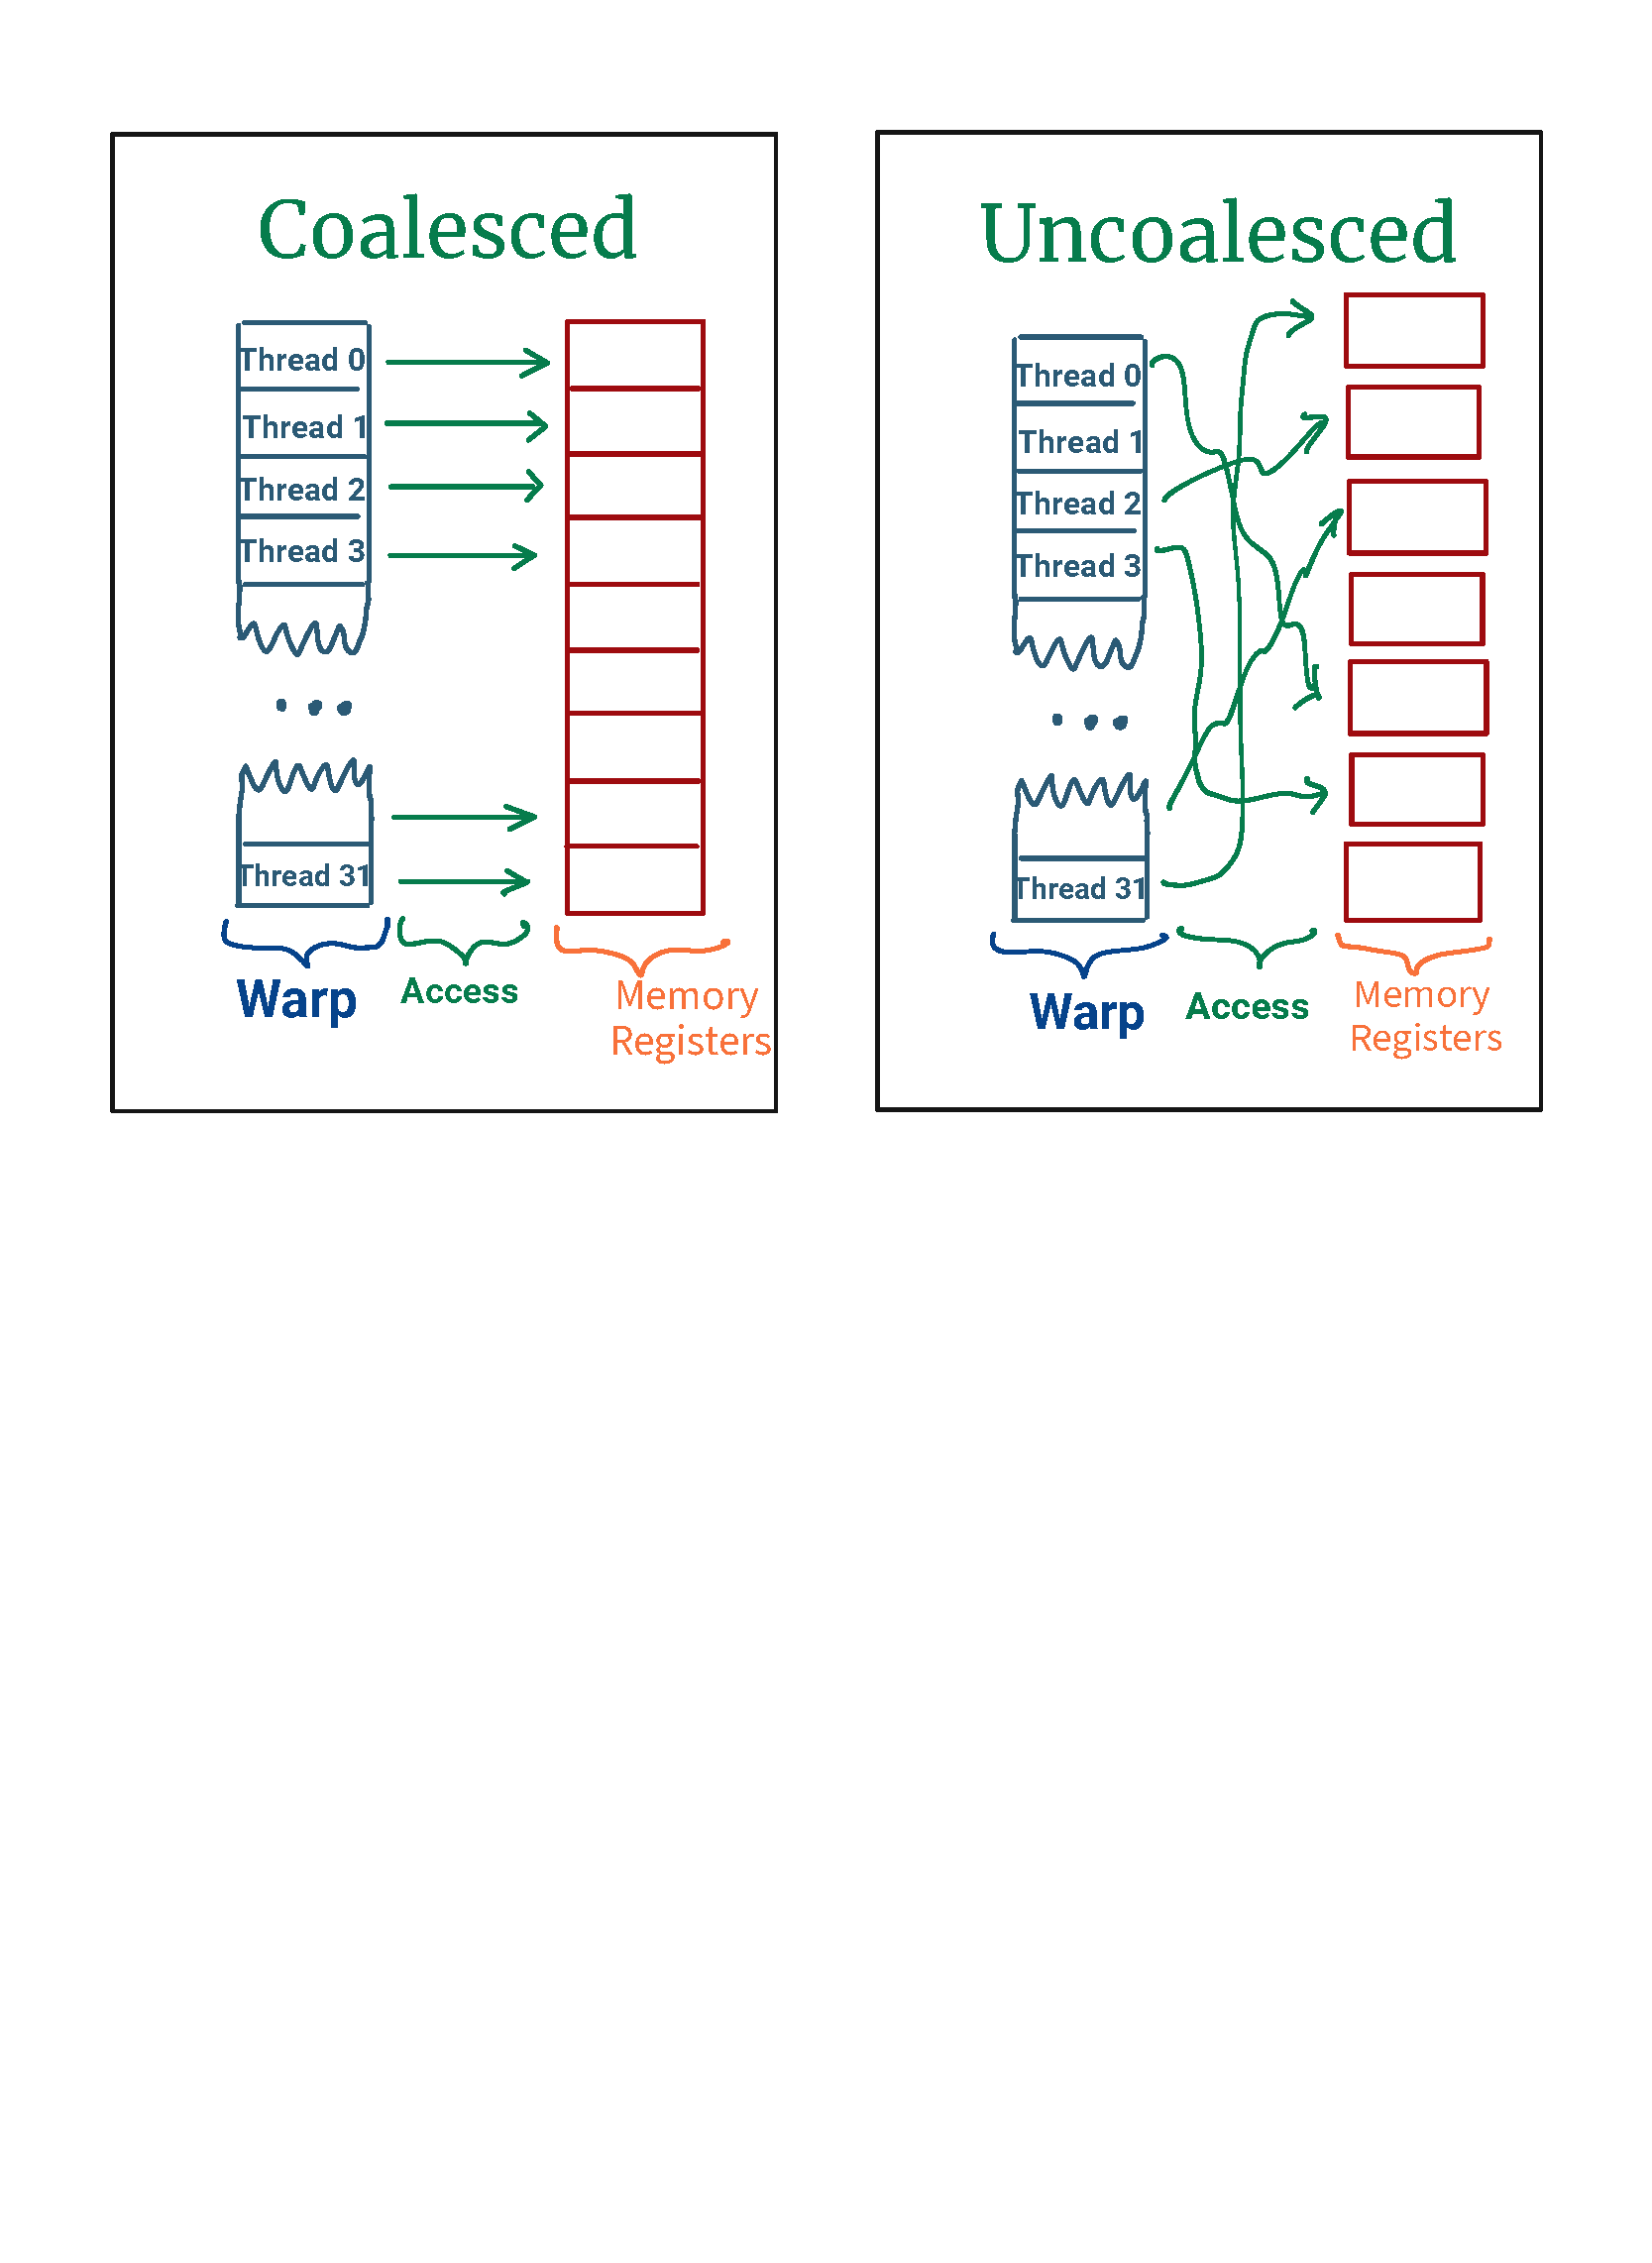
\includegraphics[height=5cm]{pngs/coalesced.png}
    %\end{center}
   \caption{Memory access optimization mechanism.}
   \label{coalesced}
\end{wrapfigure}

Imagine a certain number of warps are scheduled by the SM. Lets say 2 blocks of 128 threads, which gives 
$2\text{blocks}\cdot\nicefrac{128\text{thr.}}{32} = 8 \text{warps}$. These warps fetch some data 
from a certain field of memory of the GPU. We know that the warp is something very grouped, even physically 
the threads are grouped in it. It would be logical that they access adjacent memory addresses. This notion 
may seem quite confusing in the beginning, but let's see how Nvidia is describing it\cite{center}:

\vspace{-10pt}
\begin{quote}
   \textsl{Global memory instructions support reading or writing words \footnote{Words can be data type of a certain size.} 
   of size equal to 1, 2, 4, 8, or 16 bytes. 
   Any access (via a variable or a pointer) to data residing in global memory compiles to a single global memory 
   instruction \textbf{if and only if} the size of the data type is 1, 2, 4, 8, or 16 bytes and the data is naturally aligned 
   (i.e., its address is a multiple of that size). If this size and alignment requirement is not fulfilled, the access 
   compiles to multiple instructions with interleaved access patterns that prevent these instructions from fully coalescing.}
\label{coalescedquote}
\end{quote}
Do not pay attention to the notion of \textbf{global} memory (we will discuss it soon).
Try to read the Nvidia standart above again by looking at the coalesced scheme (\autoref{coalesced})
to fully understand the mechanism. One may notice that this notion is crucial in the performance of the code.
Indeed, when writing the kernel, one must keep in mind this aspect and try to ensure (\sout{when possible}) 
a coalesced memory access.

\vspace{-15pt}
\paragraph{\underline{Global memory}} is the largest memory in terms of the size, and yet with the greatest latency.
As we've discussed, the kernels are launched \textbf{from} the CPU. It would be wise to be able to share 
resources between the host and the device. For example, send data to the GPU from a usual \verb|C| programm
and retrieve back in a processed form. This is exactly the purpose of the global memory. The global memory, as the 
name suggests is \textsl{global}, i.e. it is \textbf{visible to all threads from all blocks}. As we will see in practice,
the usual workflow is to copy the data from the global memory to some other (which is discussed below), 
which is faster \footnote{You may think of it as the {\fontfamily{pcr}\selectfont malloc()} or {\fontfamily{pcr}\selectfont calloc()} functions in C
or the keyword {\fontfamily{pcr}\selectfont new} in C++. Indeed, the allocation and the access to those variables is slower than 
declaring on the stack:\newline {\fontfamily{pcr}\selectfont int $^{\ast}$ ptr\_a = new int; } is slower than {\fontfamily{pcr}\selectfont int a = \{\};}}  
to manipulate. 

\vspace{-15pt}
\paragraph{\underline{Shared memory}} \label{grocery_store} is much faster than the global one, but evidently smaller. Other 
crucial difference is the scope - the shared memory is \textbf{only seen by threads in the same block}. This provides 
the ability for threads to share results and temporary calculations, and process the data \textsc{in place}. 
Think of this situation as a client of a grocery store, where the customers are sort of threads. Every time a person 
wants to cook something at their house, they don't drive to the store to buy every ingredient. They rather go there 
once a week, for example, and buy the amount they need. They also make sure, 
that everything can fit in the fridge. Thus 
in this \sout{wonderful} analogy, the fridge is the low latency shared memory, and the grocery shop - the 
big and unwieldy global resource.
One sometimes refer to this memory as 
\textsl{cache memory controlled by the programmer}. However, it is important to take note that the reduced 
latency of the shared memory does not guarantee a better performance. Indeed, the biggest pitfall for all \sout{of us} beginners 
are the \textit{bank conflicts}\footnote{A small disclaimer: the notion of \textit{bank conflicts} was one of the reasons for these personal 
notes. The reader should not panic if he's missing something. The examples will be discussed later in the practice part. So one 
should, if necessary, come back to this "theoretical" part after going through the examples. \sout{The author wants to apologize 
for the eventual wordiness.}}. 

\paragraph{Bank conflicts.}We already discussed the notion of warps, as an execution entity encapsulating threads. 
One may think of the \underline{bank conflicts} as the analogy of warps in memory
 (i.e. warps are located at the \textit{execution level abstraction}, and the 
 bank conflicts-at the \textit{memory level abstraction}). 
 Shared memory is organized into \underline{banks}.
One \textit{layer bank} is a sequential field of 32 memory adreses of 4 bits ($32\text{\#adreses}\cdot 4\text{bits}$). 

\begin{quote}
   \textsl{Memory can serve as many simultaneous address as it has banks.} 
\end{quote}
This is a very important property, so lest's consider an another \sout{illustrative} analogy. Suppose in a restaurant, each waiter 
is assigned a strict number of tables, such that a waiter $A$ cannot take $B$'s tables. Suppose you are the host at this restaurant, 
and you have a large group of people, who's number is the exact number as the resaurant's seats. The wise choice would be to 
partition them between all the waiter's assigned tables, right? Wouldn't that be silly to partition all the guests, excepting one, 
who will be waiting for a free place at $A$'s waiter's table, while there are free places at $B$'s table? The analogy \sout{may} not be 
the best, but the sketch should do the trick: 

\begin{figure}[H]
   \centering
   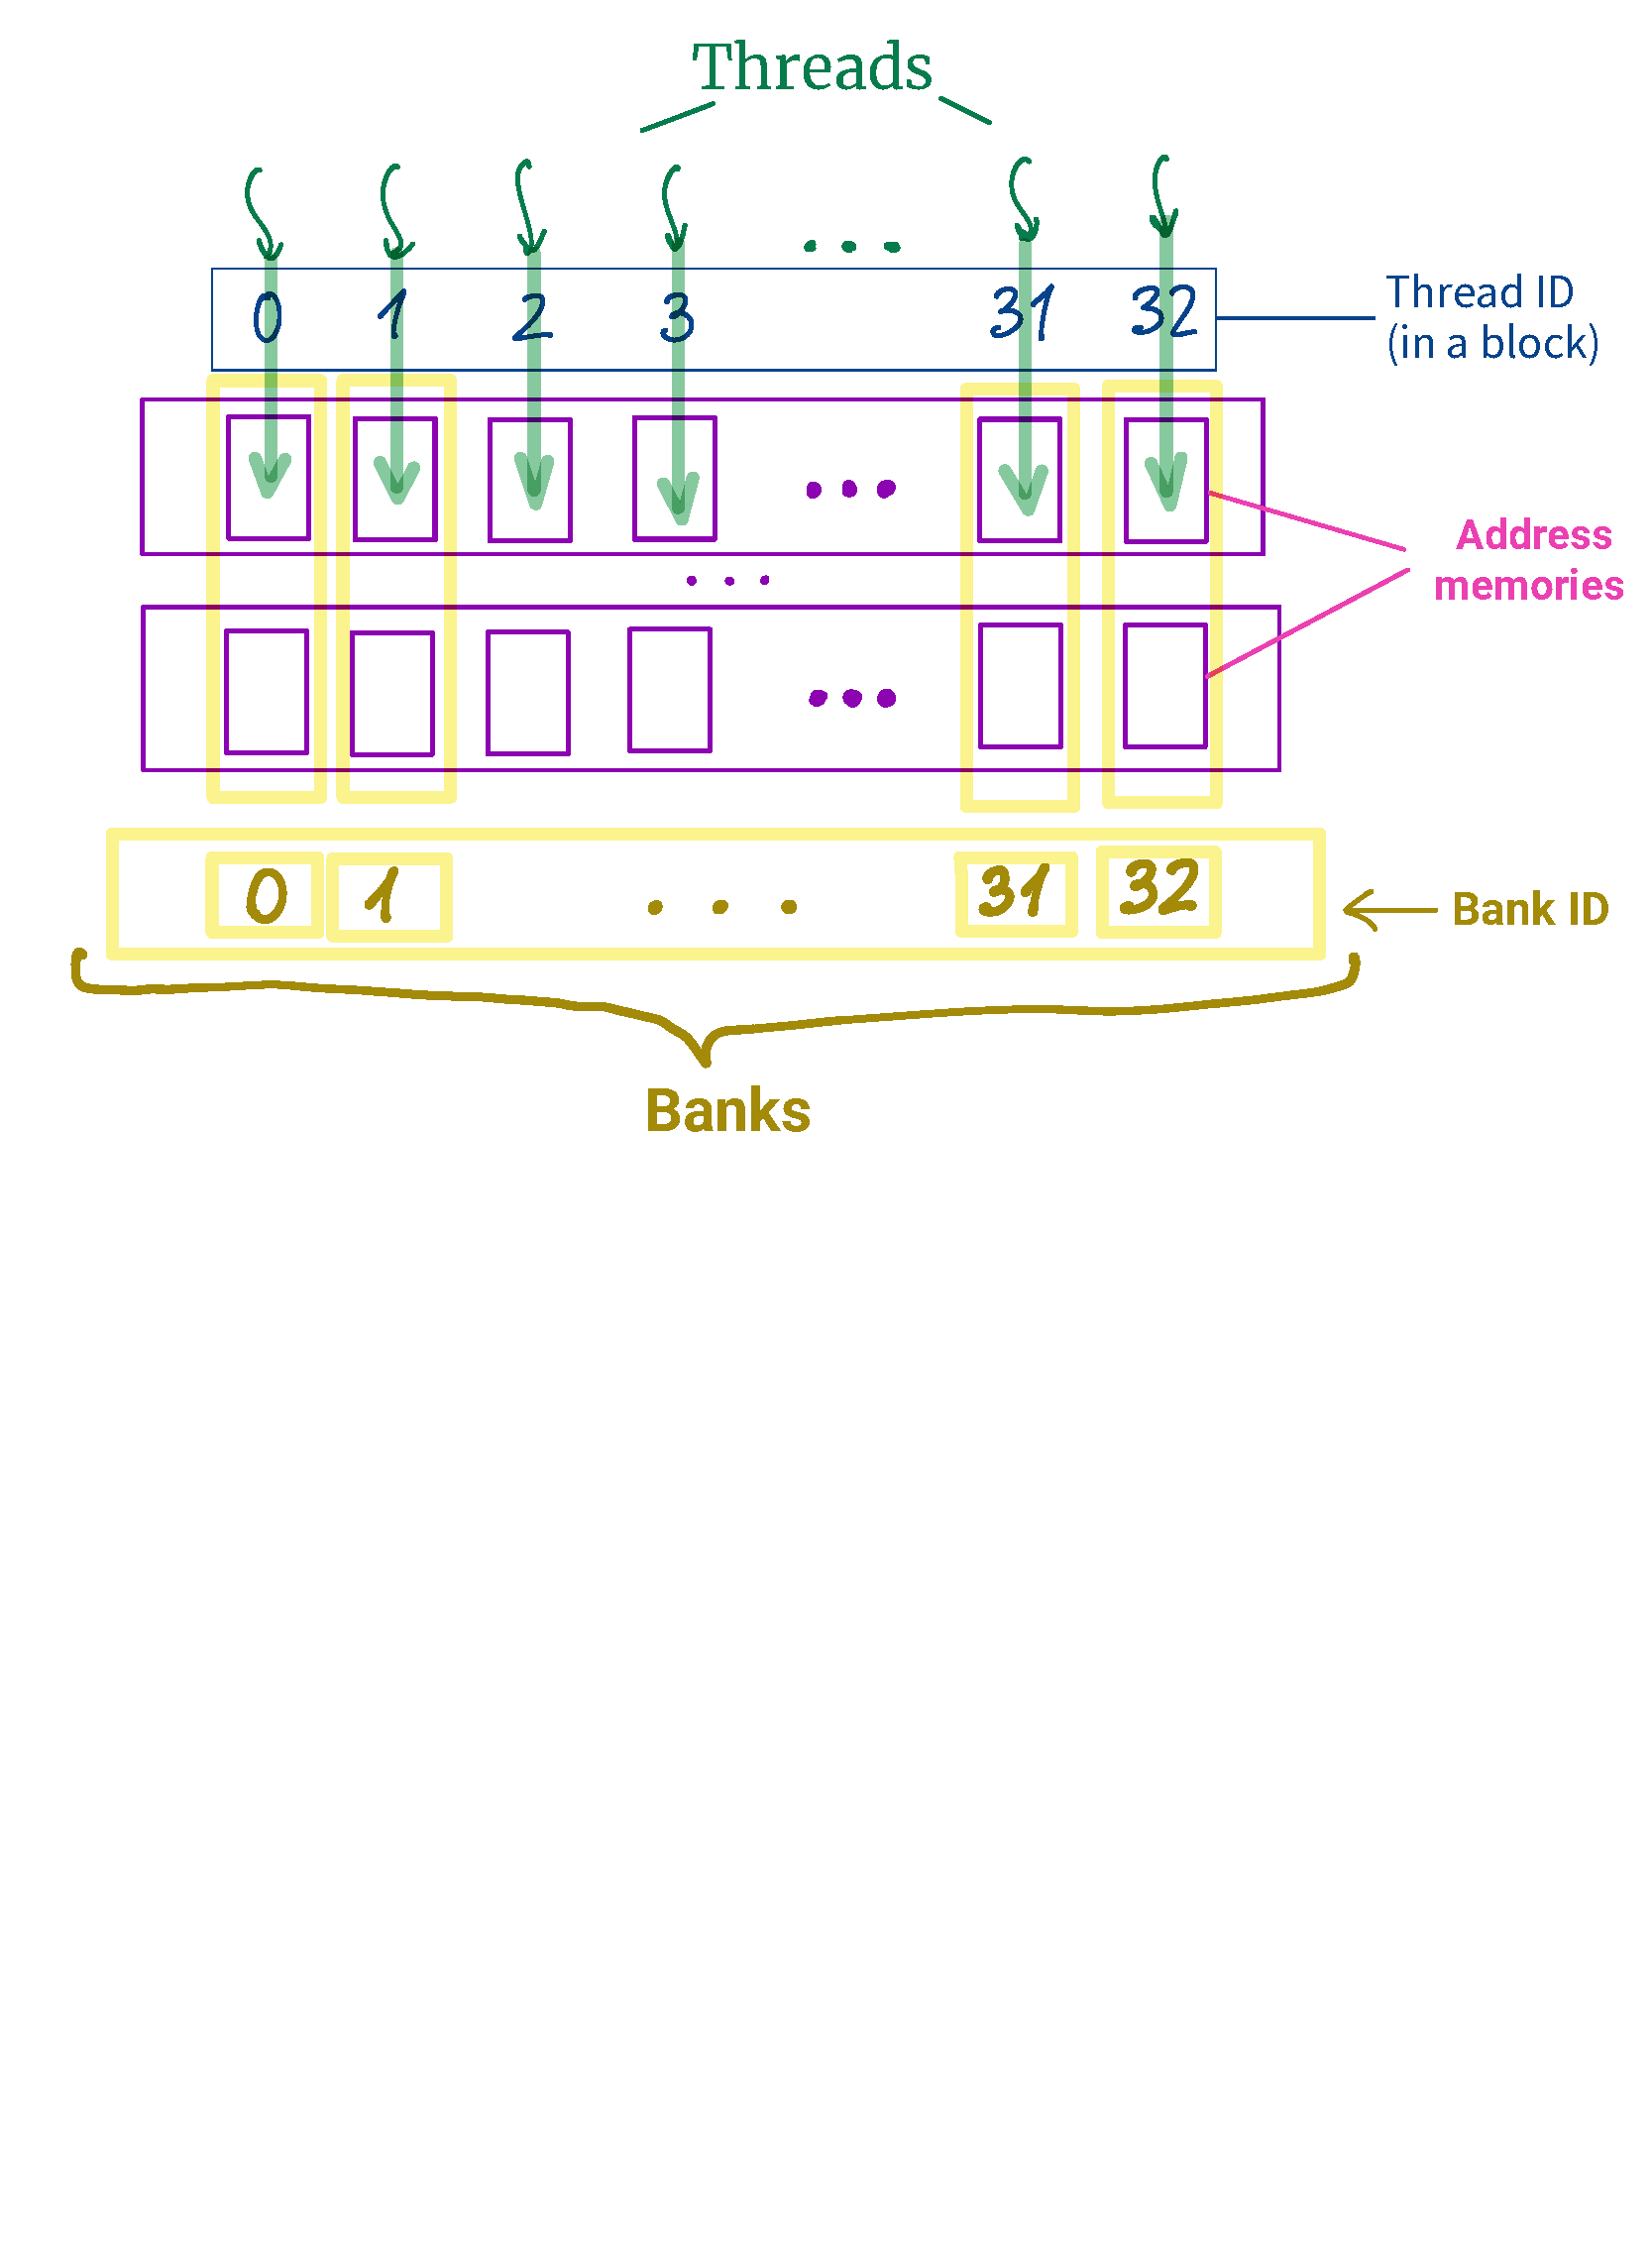
\includegraphics[scale=0.18]{pngs/banks1.png}
   \caption{Memory banks serving the threads. Only one thread can access a bank with a certain ID simultaneously. 
   From the analogy, threads are clients, and banks are waiters, giving them memory.}
   \label{banks}

\end{figure}

\vspace{-0.5cm}
\paragraph{Read-only memory$\ast$} is, as its name suggests, can't be changed by the kernel's threads, but is loaded at compile time. This memory is not as commonly 
described in the GPGPU programming documentation. It is often 
encapsulated in the GPU APIs, such as OpenGL. Thus by using those API's, the programming is indirectly 
reffered as the read-only memory.

\paragraph{Local registers}By looking at the scheme of the architecture of the GPU vs the CPU (\autoref{cpuvsgpu}), one may notice the amount 
of registers in the GPU vs the CPU. The amount of registers in the GPU
is incomprarble with the registers of the CPU. As you might have guessed, a 
register is memory, with the scope of a thread. The compiler of a CUDA program will try to optimize the number and size of registers. 
It is nevertheless possible, that the amount of memory in registers may fall short. Then the L1 and/or L2 caches will enter the 
play. This is the fastest memory available in the CUDA API, yet the most restrictive.

\subsection{Memory allocation model}
\label{subsection:mem_alloc_model}
By now, we've made the difference between kinds of memory in terms of the scope, i.e, 
\textbf{who} and \textbf{when} is able to access various kinds of memory. This, of course, somehow impacts the way we're allocating it. 
However, one can classify the memory, in terms of its \textbf{allocation}. There are mainly fours ways of memory allocation.


We will see further that standart 
code, which uses GPU resources, follows a certain path/pipeline. 
Roughly that is: 
\begin{enumerate}
\setlength\itemsep{-0.1em}
  \item Resource declaration on the host (using \verb|malloc|) and initialization using \verb|memcpy|.
  \item Memory allocation and initialization on the device.
  \item Memory copying/transfer from the host to device.
  \item Accelerated computation on the GPU and storage of the results fro the device
  \item Copy of data from the device back to the host.
\end{enumerate}

One of the steps is the allocation of 
memory on the GPU from the host (by calling a certain CUDA function, which will be described later). 
\begin{itemize}
\setlength\itemsep{-0.1em}
   \item Pageable memory
   \item Pinned memory
   \item Mapped memory
   \item Unified memory
\end{itemize}
The difference in terms of the API calls, use cases and mechanisms, will be explained further. 

















